\documentclass{article}
\usepackage{polski}
\usepackage[utf8]{inputenc}
\usepackage[a4paper, total={6in, 10in}]{geometry}
\usepackage{graphicx}
\usepackage{float}
\usepackage{pgfplotstable}
\usepackage{booktabs}
\usepackage{ragged2e}
\usepackage{caption}
\usepackage{subcaption}
\usepackage{algorithm}
\usepackage{algpseudocode}
\usepackage{amsmath}
\usepackage{adjustbox}
\usepackage{tabularx}
\title{Sprawozdanie Lista 4}
\author{Tymoteusz Roźmiarek}
\renewcommand{\algorithmicrequire}{\textbf{Input:}}
\renewcommand{\algorithmicensure}{\textbf{Output:}}

\begin{document}
\maketitle
\justifying

\section*{Maksymalny przepływ}
\textbf{Sieć rezydualna} to graf reprezentujący, ile dodatkowego przepływu można przesłać przez sieć przepływową, biorąc pod uwagę istniejący przepływ. Dla krawędzi z przepływem, pojemność rezydualna jest różnicą między oryginalną pojemnością a aktualnym przepływem.\\
\textbf{Ścieżka powiększająca} to ścieżka w sieci rezydualnej z węzła źródłowego do węzła ujścia, wzdłuż której można zwiększyć przepływ. Zwiększenie przepływu wzdłuż ścieżki powiększającej oznacza dodanie pewnej wartości do przepływu na każdej krawędzi tej ścieżki.\\
\\
\textbf{Algorytm Edmondsa-Karpa} jest odmianą algorytmu Forda-Fulkersona do znajdowania maksymalnego przepływu w sieci przepływowej. Działa on poprzez wielokrotne znajdowanie ścieżki powiększającej w sieci rezydualnej i zwiększanie przepływu wzdłuż tej ścieżki. W przeciwieństwie do ogólnego algorytmu Forda-Fulkersona, algorytm Edmondsa-Karpa zawsze wybiera najkrótszą ścieżkę powiększającą, gdzie długość jest mierzona liczbą krawędzi. To ograniczenie gwarantuje, że algorytm zakończy się w czasie wielomianowym.
Algorytm można podsumować następująco:
\begin{enumerate}
\item Inicjalizacja: Ustaw przepływ na każdej krawędzi na 0.
\item Pętla: Dopóki istnieje ścieżka powiększająca w sieci rezydualnej:
\begin{itemize}
\item Znajdź najkrótszą ścieżkę powiększającą za pomocą przeszukiwania wszerz (BFS).
\item Zwiększ przepływ wzdłuż tej ścieżki o maksymalną możliwą wartość.
\item Zaktualizuj sieć rezydualną.
\end{itemize}
\item Zwróć znaleziony przepływ.
\end{enumerate}
Algorytm Edmondsa-Karpa ma złożoność czasową $O(nm^2)$, gdzie $n$ to liczba węzłów, a $m$ to liczba krawędzi w sieci.
\subsection*{Wyniki}
\begin{figure}[H]
    \centering
    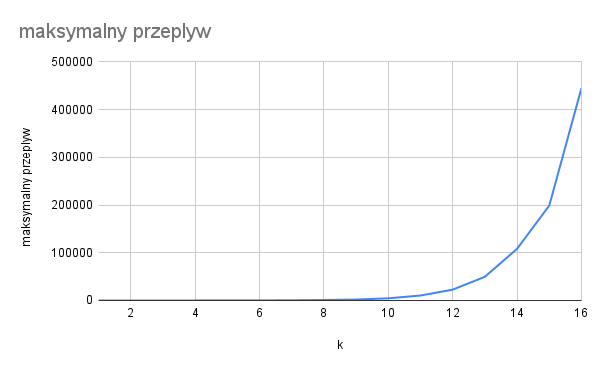
\includegraphics[width=0.7\textwidth]{max\_flow/przeplyw.png}
    \caption{Maksymalny przepływ w zależności od $k$}
\end{figure}
\begin{figure}[H]
    \centering
    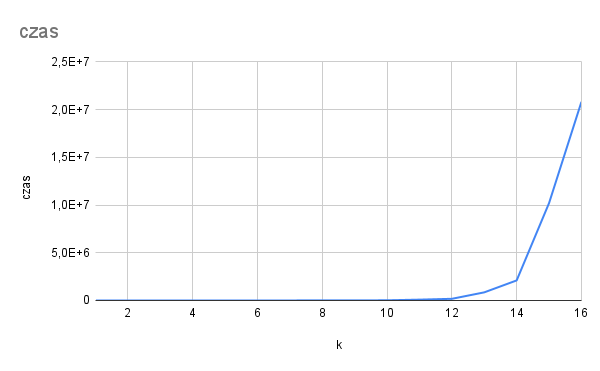
\includegraphics[width=0.7\textwidth]{max\_flow/czas.png}
    \caption{Czas działania programu w zależności od $k$ (w mikrosekundach)}
\end{figure}
\begin{figure}[H]
    \centering
    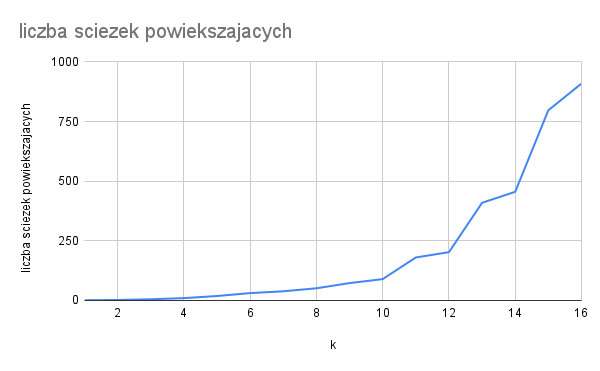
\includegraphics[width=0.7\textwidth]{max\_flow/sciezek.png}
    \caption{Liczba ścieżek powiększających w zależności od $k$}
\end{figure}

\section*{Skojarzenie o największym rozmiarze}
Do rozwiązania wykorzystałem \textbf{algorytm Hopcroft-Karp} . Jest to ulepszenie w stosunku do algorytmu Edmondsa-Karpa. W przypadku grafów dwudzielnych, problem maksymalnego dopasowania można przekształcić w problem maksymalnego przepływu, ale algorytm Hopcroft-Karp działa szybciej. Algorytm Hopcroft-Karp opiera się na koncepcji sieci rezydualnej i ścieżek powiększających, podobnie jak algorytm Edmondsa-Karpa. W sieci rezydualnej dla grafu dwudzielnego, każda ścieżka powiększająca ma długość co najmniej 2 (ponieważ musi przechodzić przez co najmniej jeden węzeł z każdego "zbioru" w grafie dwudzielnym). Algorytm Hopcroft-Karp wykorzystuje ten fakt, aby w każdej fazie znajdować maksymalny zbiór ścieżek powiększających o minimalnej długości, które nie mają ze sobą wspólnych węzłów. Zwiększa on przepływ wzdłuż wszystkich ścieżek w tym zbiorze jednocześnie, co przyspiesza proces znajdowania maksymalnego dopasowania.\\
Algorytm można podsumować następująco:
\begin{enumerate}
\item Inicjalizacja: Ustaw dopasowanie na puste.
\item Pętla: Dopóki istnieje ścieżka powiększająca w sieci rezydualnej:
\begin{itemize}
\item Znajdź maksymalny zbiór rozłącznych ścieżek powiększających o minimalnej długości.
\item Zwiększ dopasowanie o wszystkie krawędzie w znalezionych ścieżkach.
\item Zaktualizuj sieć rezydualną.
\end{itemize}
\item Zwróć maksymalne skojarzenie.
\end{enumerate}
Algorytm Hopcroft-Karp ma złożoność czasową $O(\sqrt{n}m)$, gdzie $n$ to liczba węzłów, a $m$ to liczba krawędzi w grafie.

\subsection*{Wyniki}
\subsubsection*{Wykresy wielkości maksymalnego skojarzenia w zaleznosci od i, dla kazdego k }
\begin{figure}[H]
\centering
\begin{minipage}{0.45\textwidth}
\centering
\includegraphics[width=\textwidth]{skoj/max\_matching\_k3.png}
\end{minipage}
\hfill
\begin{minipage}{0.45\textwidth}
\centering
\includegraphics[width=\textwidth]{skoj/max\_matching\_k4.png}
\end{minipage}
\end{figure}
\begin{figure}[H]
\centering
\begin{minipage}{0.45\textwidth}
\centering
\includegraphics[width=\textwidth]{skoj/max\_matching\_k5.png}
\end{minipage}
\hfill
\begin{minipage}{0.45\textwidth}
\centering
\includegraphics[width=\textwidth]{skoj/max\_matching\_k6.png}
\end{minipage}
\end{figure}
\begin{figure}[H]
\centering
\begin{minipage}{0.45\textwidth}
\centering
\includegraphics[width=\textwidth]{skoj/max\_matching\_k7.png}
\end{minipage}
\hfill
\begin{minipage}{0.45\textwidth}
\centering
\includegraphics[width=\textwidth]{skoj/max\_matching\_k8.png}
\end{minipage}
\end{figure}
\begin{figure}[H]
\centering
\begin{minipage}{0.45\textwidth}
\centering
\includegraphics[width=\textwidth]{skoj/max\_matching\_k9.png}
\end{minipage}
\hfill
\begin{minipage}{0.45\textwidth}
\centering
\includegraphics[width=\textwidth]{skoj/max\_matching\_k10.png}
\end{minipage}
\end{figure}

\subsubsection*{Wykresy wykresy czasu działania programu w zależności od k, dla każdego i}
\begin{figure}[H]
\centering
\begin{minipage}{0.45\textwidth}
\centering
\includegraphics[width=\textwidth]{skoj/time\_i1.png}
\end{minipage}
\hfill
\begin{minipage}{0.45\textwidth}
\centering
\includegraphics[width=\textwidth]{skoj/time\_i2.png}
\end{minipage}
\end{figure}
\begin{figure}[H]
\centering
\begin{minipage}{0.45\textwidth}
\centering
\includegraphics[width=\textwidth]{skoj/time\_i3.png}
\end{minipage}
\hfill
\begin{minipage}{0.45\textwidth}
\centering
\includegraphics[width=\textwidth]{skoj/time\_i4.png}
\end{minipage}
\end{figure}
\begin{figure}[H]
\centering
\begin{minipage}{0.45\textwidth}
\centering
\includegraphics[width=\textwidth]{skoj/time\_i5.png}
\end{minipage}
\hfill
\begin{minipage}{0.45\textwidth}
\centering
\includegraphics[width=\textwidth]{skoj/time\_i6.png}
\end{minipage}
\end{figure}
\begin{figure}[H]
\centering
\begin{minipage}{0.45\textwidth}
\centering
\includegraphics[width=\textwidth]{skoj/time\_i7.png}
\end{minipage}
\hfill
\begin{minipage}{0.45\textwidth}
\centering
\includegraphics[width=\textwidth]{skoj/time\_i8.png}
\end{minipage}
\end{figure}

\section*{Modele programowania liniowego}
\subsection*{Model dla zadania znajdowania maksymalnego przepływu:}
\begin{align*}
    & \text{Zbiór wierzchołków:} & V \\
    & \text{Zbiór krawędzi:} & E \subseteq V \times V \\
    & \text{Pojemność krawędzi:} & c_{ij} \geq 0, \quad \forall (i,j) \in E \\
    & \text{Wierzchołek źródłowy:} & s \geq 0 \\
    & \text{Wierzchołek ujścia:} & t > 0 \\
    & \text{Przepływ po krawędzi:} & f_{ij} \geq 0, \quad \forall (i,j) \in E \\
\end{align*}
Problem maksymalnego przepływu:
\begin{align*}
    \text{maksymalizuj} \quad & \sum_{(s,j) \in E} f_{sj} \\
    \text{pod warunkiem że} \quad & f_{uv} \leq c_{uv}, \quad \forall (u,v) \in E \\
    & \sum_{u \in V: (u,v) \in E} f_{uv} = \sum_{w \in V: (v,w) \in E} f_{vw}, \quad \forall v \in V \setminus \{s,t\}
\end{align*}

\subsection*{Wyniki}
\begin{table}[H]
\centering
\caption{Porównanie wyników algorytmu C++ i solvera dla $k=2$}
\begin{tabular}{lcc}
\toprule
Parametr                   & C++ (s) & Solver (s) \\
\midrule
Maksymalny przepływ       & 5      & 5       \\
Czas (s)                      & 0.0    & 0.0    \\
\bottomrule
\end{tabular}
\end{table}

\begin{table}[H]
\centering
\caption{Porównanie wyników algorytmu C++ i solvera dla $k=7$}
\begin{tabular}{lcc}
\toprule
Parametr                   & C++ (s) & Solver (s) \\
\midrule
Maksymalny przepływ       &  339     &  339   \\
Czas (s)                     & 0.0    & 0.0    \\
\bottomrule
\end{tabular}
\end{table}

\begin{table}[H]
\centering
\caption{Porównanie wyników algorytmu C++ i solvera dla $k=13$}
\begin{tabular}{lcc}
\toprule
Parametr                   & C++ (s) & Solver (s) \\
\midrule
Maksymalny przepływ       &  44555     &  44555   \\
Czas (s)                     & 0.809    & 7.8    \\
\bottomrule
\end{tabular}
\end{table}

\begin{table}[h]
\centering
\caption{Przepływy po krawędziach C++ i Solver dla $k=2$}
\begin{minipage}{0.45\textwidth}
\centering
\begin{tabular}{|l|c|}
\hline
Krawędź                   & Przepływ (C++) \\
\hline
0 $\to$ 1 & 1\\
0 $\to$ 2& 2\\
1 $\to$ 3& 1\\
2 $\to$ 3& 2\\
\hline
\end{tabular}
\end{minipage}
\hfill
\begin{minipage}{0.45\textwidth}
\centering
\begin{tabular}{|l|c|}
\hline
Krawędź                   & Przepływ (Solver) \\
\hline
0 $\to$ 1 & 1\\
0 $\to$ 2& 2\\
1 $\to$ 3& 1\\
2 $\to$ 3& 2\\
\hline
\end{tabular}
\end{minipage}
\end{table}

\begin{table}[h]
\centering
\caption{Przepływy po krawędziach C++ i Solver dla $k=3$}
\begin{minipage}{0.45\textwidth}
\centering
\begin{tabular}{|l|c|}
\hline
Krawędź                   & Przepływ (C++) \\
\hline
0 $\to$ 1 & 3\\
0 $\to$ 2& 2\\
0 $\to$ 4& 3\\
1 $\to$ 3& 3\\
1 $\to$ 5& 0\\
2 $\to$ 3& 0\\
2 $\to$ 6& 2\\
3 $\to$ 7& 3\\
4 $\to$ 5& 2\\
4 $\to$ 6& 1\\
5 $\to$ 7& 2\\
6 $\to$ 7& 3\\
\hline
\end{tabular}
\end{minipage}
\hfill
\begin{minipage}{0.45\textwidth}
\centering
\begin{tabular}{|l|c|}
\hline
Krawędź                   & Przepływ (Solver) \\
\hline
0 $\to$ 1 & 3\\
0 $\to$ 2& 2\\
0 $\to$ 4& 3\\
1 $\to$ 3& 3\\
1 $\to$ 5& 0\\
2 $\to$ 3& 0\\
2 $\to$ 6& 2\\
3 $\to$ 7& 3\\
4 $\to$ 5& 2\\
4 $\to$ 6& 1\\
5 $\to$ 7& 2\\
6 $\to$ 7& 3\\
\hline
\end{tabular}
\end{minipage}
\end{table}

\subsection*{Model dla zadania znajdowania największego skojarzenia:}
\begin{align*}
    &\text{Zbiory wierzchołków:} & U, V \\
    &\text{Macierz sąsiedztwa:} & e_{uv} \in \{0, 1\}, \quad \forall u \in U, v \in V \\
    &\text{Zmienna decyzyjna:} & x_{uv} \in \{0, 1\}, \quad \forall u \in U, v \in V \\
\end{align*}

Problem maksymalnego skojarzenia:
\begin{align*}
    \text{maksymalizuj} \quad & \sum_{u \in U} \sum_{v \in V} x_{uv} \\
    \text{pod warunkiem że} \quad & \sum_{v \in V} x_{uv} \leq 1, \quad \forall u \in U \\
    & \sum_{u \in U} x_{uv} \leq 1, \quad \forall v \in V \\
    & x_{uv} \leq e_{uv}, \quad \forall u \in U, v \in V
\end{align*}

\subsection*{Wyniki}
\begin{table}[H]
\centering
\caption{Porównanie wyników algorytmu C++ i solvera dla $k=4,$, $i=2$}
\begin{tabular}{lcc}
\toprule
Parametr                   & C++ (s) & Solver (s) \\
\midrule
Maksymalne skojarzenie & 13      & 13       \\
Czas (s)                      & 0.0    & 0.0    \\
\bottomrule
\end{tabular}
\end{table}

\begin{table}[H]
\centering
\caption{Porównanie wyników algorytmu C++ i solvera dla $k=8, i=4$}
\begin{tabular}{lcc}
\toprule
Parametr                   & C++ (s) & Solver (s) \\
\midrule
Maksymalny przepływ       & 248      & 248       \\
Czas (s)                      & 0.003    & 0.7    \\
\bottomrule
\end{tabular}
\end{table}

\begin{table}[H]
\centering
\caption{Porównanie wyników algorytmu C++ i solvera dla $k=10, i=5$}
\begin{tabular}{lcc}
\toprule
Parametr                   & C++ (s) & Solver (s) \\
\midrule
Maksymalny przepływ       & 1016      &  1016       \\
Czas (s)                      & 0.025    &  	82.8    \\
\bottomrule
\end{tabular}
\end{table}

\begin{table}[H]
\centering
\begin{minipage}{0.45\textwidth}
\centering
\begin{tabular}{|l|c|}
\hline
C++ & Solver\\
\hline
(0, 1)&(0, 1)\\
(1, 0)&(1, 0)\\
(3, 2)&(3, 2)\\
\hline
\end{tabular}
\caption{$k=2,i=1$}
\end{minipage}
\hfill
\begin{minipage}{0.45\textwidth}
\centering
\begin{tabular}{|l|c|}
\hline
C++ & Solver\\
\hline
(0, 1)&(0, 1)\\
(1, 6)&(1, 6)\\
(2, 3)&(2, 3)\\
(3, 0)&(3, 0)\\
(4, 4)&(4, 4)\\
(6, 7)&(6, 7)\\
(7, 5)&(7, 5)\\
\hline
\end{tabular}
\caption{$k=3,i=2$ }
\end{minipage}
\end{table}

\begin{table}[H]
\centering
\begin{tabular}{|l|c|}
\hline
C++ & Solver\\
\hline
(0, 4) & (0, 4)\\
(1, 2) & (1, 2)\\
(2, 3) &(2, 3)\\
(3, 13)& (3, 13)\\
(4, 5) &(4, 5)\\
(6, 11)& (6, 11)\\
(7, 0) &(7, 0)\\
(8, 8) &(8, 8)\\
(9, 10)& (9, 10)\\
(10, 6)& (10, 6)\\
(11, 9)& (11, 9)\\
(12, 7)& (12, 7)\\
(13, 12)& (13, 12)\\
(15, 1) &(15, 1)\\
\hline
\end{tabular}
\caption{$k=4,i=2$ }
\end{table}

\section*{Algorytm Dynica}
\textbf{Sieć warstwowa} składa się z warstw węzłów, gdzie warstwa 0 to węzeł źródłowy, a warstwa k to zbiór węzłów, do których można dotrzeć z węzła źródłowego w dokładnie k krokach w sieci rezydualnej.\\
\textbf{Algorytm Dynica} jest algorytmem służącym do znajdowania maksymalnego przepływu w sieci przepływowej. Działa on poprzez budowanie sieci warstwowej, która jest podgrafem sieci rezydualnej, i znajdowanie w niej ścieżek powiększających. Algorytm Dynica wyszukuje ścieżki powiększające w sieci warstwowej, dopóki nie będzie już możliwe dotarcie do węzła ujścia. Wtedy buduje nową sieć warstwową i powtarza proces.\\
Algorytm można podsumować następująco:
\begin{enumerate}
\item Inicjalizacja: Ustaw przepływ na każdej krawędzi na 0.
\item Pętla: Dopóki istnieje ścieżka z węzła źródłowego do węzła ujścia w sieci rezydualnej:
\begin{itemize}
\item Zbuduj sieć warstwową.
\item Znajdź ścieżki powiększające w sieci warstwowej i zwiększ przepływ wzdłuż tych ścieżek.
\end{itemize}
\item Zwróć znaleziony przepływ.
\end{enumerate}
Algorytm Dynica ma złożoność czasową $O(n^2m)$, gdzie $n$ to liczba węzłów, a $m$ to liczba krawędzi w sieci. W praktyce algorytm Dynica często działa szybciej, szczególnie w przypadku gęstych sieci.

\subsection*{Wyniki}
\begin{figure}[H]
    \centering
    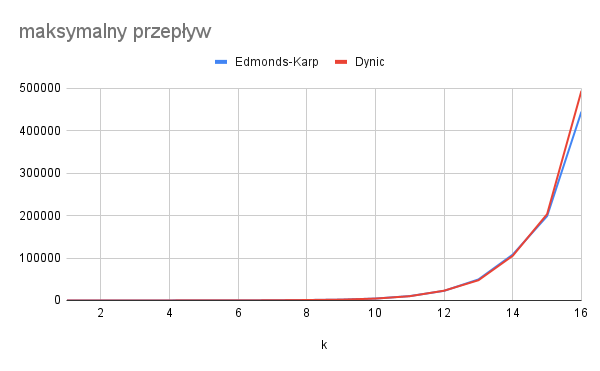
\includegraphics[width=0.7\textwidth]{dynic/przep.png}
    \caption{Maksymalny przepływ w zależności od $k$}
\end{figure}
\begin{figure}[H]
    \centering
    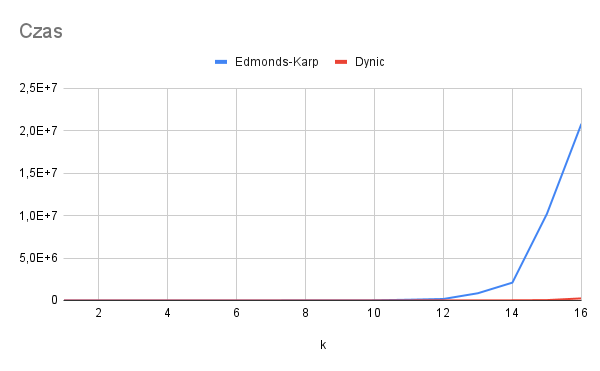
\includegraphics[width=0.7\textwidth]{dynic/czas.png}
    \caption{Czas działania programu w zależności od $k$ (w mikrosekundach)}
\end{figure}
\begin{figure}[H]
    \centering
    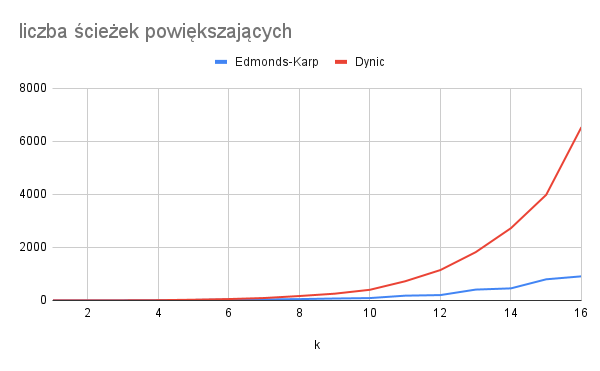
\includegraphics[width=0.7\textwidth]{dynic/sciez.png}
    \caption{Liczba ścieżek powiększających w zależności od $k$}
\end{figure}
Na powyższych wykresach widać, że algorytm Dynica działa o wiele szybciej niż algorytm Edmondsa-Karpa. Różnica robi się bardzo zauważalna dla $k \geq 12$. Ponadto algorytm Dynica wykorzystuje zdecydowanie więcej ścieżek powiększających.


\end{document}
